\section{Angriffe}

Das komplette Material zur vierten Aufgabe kann 
\href{https://mega.nz/file/eowBnR7S#zkweNT06YMPYXd2LO1Fy8ez1JB2mdKL_-5aUbluQVcU}
{hier} runtergeladen werden.

\subsection*{Eavsdropping Attack}

Mit folgendem Befehl wurden die Messdaten konkateniert (ohne LF):
\begin{python}
python konk_data.py -A 1_ohneBwg_A_B.csv 2_mBwg_A_B.csv 3.a_mBwg_A_B.csv 
3.a_ohneBwg_A_B.csv 3.b_mBwg_A_B.csv 3.b_ohneBwg_A_B.csv 4_mBwg_A_B.csv 
5_mBwg_A_B.csv -B 1_ohneBwg_B_A.csv 2_mBwg_B_A.csv 3.a_mBwg_B_A.csv 
3.a_ohneBwg_B_A.csv 3.b_mBwg_B_A.csv 3.b_ohneBwg_B_A.csv 4_mBwg_B_A.csv 
5_mBwg_B_A.csv -E 1_ohneBwg_E_A.csv 2_mBwg_E_A.csv 3.a_mBwg_E_A.csv
3.a_ohneBwg_E_A.csv 3.b_mBwg_E_A.csv 3.b_ohneBwg_E_A.csv 4_mBwg_E_A.csv
5_mBwg_E_A.csv
\end{python}





Folgende Befehle wurden zum Testen des Frameworks benutzt.


\begin{python}
python physec_praktikum.py -A A.csv -B B.csv -E E.csv -X 2 -Q 0
python physec_praktikum.py -A A.csv -B B.csv -E E.csv -X 2 -Q 1
\end{python}




\subsubsection*{Quantisierer im direkten Vergleich}
Schaut man sich Abbildungen~\ref{fig:4.1} und ~\ref{fig:4.2} an, 
so erkennt man merkbare Unterschiede zwischen beiden 
\textit{Quantisierern}.    

\begin{figure}[hbt!]
	\centering
		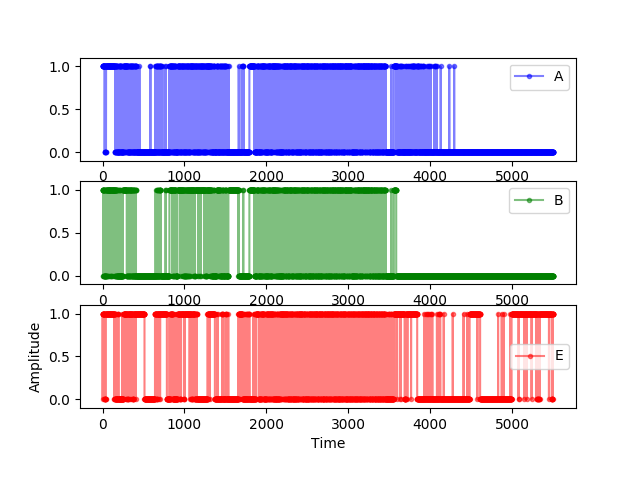
\includegraphics[width=0.65\textwidth ]
		{Bilder/a4-q0-2.png}
		\caption{\textit{quant0}}
		\label{fig:4.1}
\end{figure}


\begin{figure}[hbt!]
	\centering
		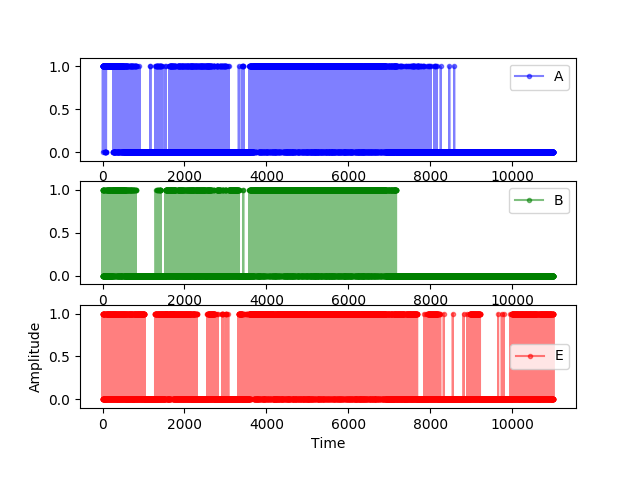
\includegraphics[width=0.65\textwidth ]
		{Bilder/a4-q1-2.png}
		\caption{\textit{quant1}}
		\label{fig:4.2}
\end{figure}


\begin{figure}[hbt!]
	\centering
		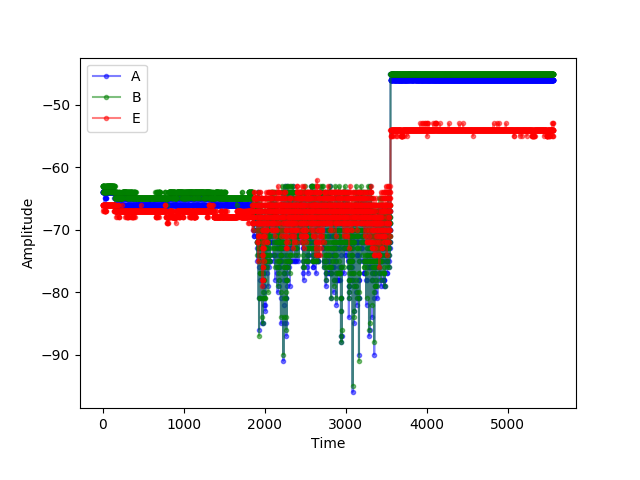
\includegraphics[width=0.65\textwidth ]
		{Bilder/a4-q0-1.png}
		\caption{\textit{Signalstärkenverlauf}}
		\label{fig:4.3}
\end{figure}

\begin{comment}
Wenn man Abbildung~\ref{fig:4.1} betrachtet, so erkennt man, 
dass Einflüsse wie Bewegung und Distanz eine große Rolle 
spielen.\\
Analysiert man die Unterschiede so wird klar, dass Bewegung
und größere Distanz einen Angreifer benachteiligen.	
\end{comment}

\newpage
Als nächstes wurde mit den Ausgaben dieses Befehls getestet.
\begin{python}
python konk_data.py -A 1_ohneBwg_A_B.csv 2_mBwg_A_B.csv -B 1_ohneBwg_B_A.csv 
2_mBwg_B_A.csv -E 1_ohneBwg_E_A.csv 2_mBwg_E_A.csv
\end{python}


\begin{figure}[hbt!]
	\centering
		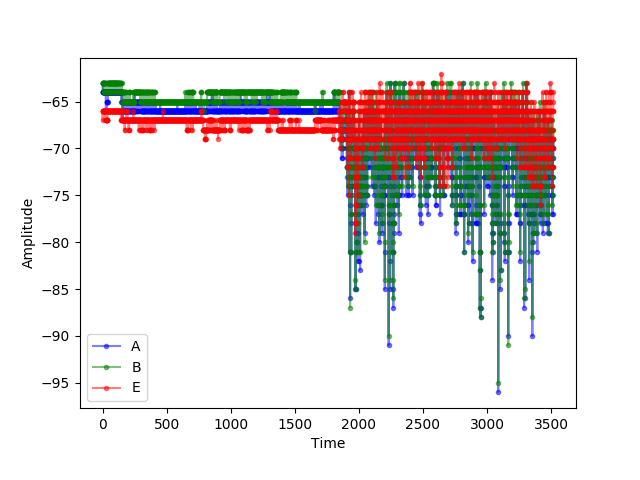
\includegraphics[width=0.65\textwidth ]
		{Bilder/a4-q0-1bis2.png}
		\caption{\textit{Signalstärkenverlauf}}
		\label{fig:4.4}
\end{figure}


\begin{figure}[hbt!]
	\centering
		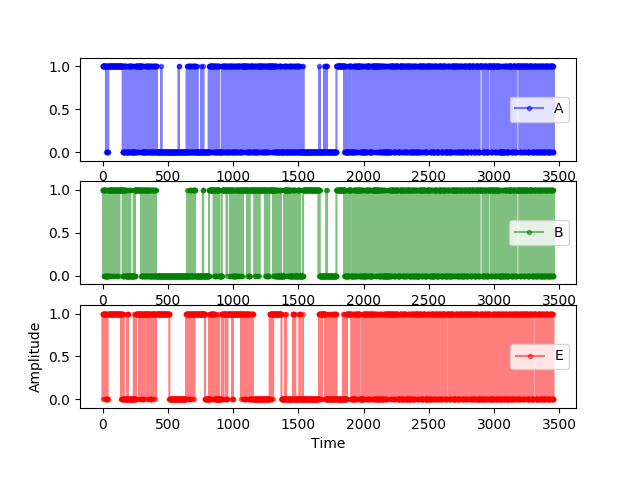
\includegraphics[width=0.65\textwidth ]
		{Bilder/a4-q0-1bis2-1.png}
		\caption{\textit{quant0}}
		\label{fig:4.5}
\end{figure}
\clearpage

\begin{figure}[hbt!]
	\centering
		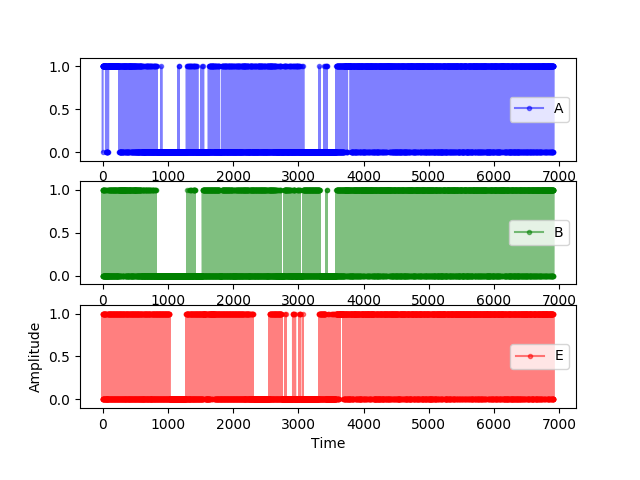
\includegraphics[width=0.65\textwidth ]
		{Bilder/a4-q1-1bis2-1.png}
		\caption{\textit{quant1}}
		\label{fig:4.6}
\end{figure}


Anschließend wurde mit den Ausgaben dieses Befehls getestet.
\begin{python}
python konk_data.py -A 3.a_mBwg_A_B.csv 3.a_ohneBwg_A_B.csv 3.b_mBwg_A_B.csv 
3.b_ohneBwg_A_B.csv  -B 3.a_mBwg_B_A.csv 3.a_ohneBwg_B_A.csv 3.b_mBwg_B_A.csv 
3.b_ohneBwg_B_A.csv -E 3.a_mBwg_E_A.csv 3.a_ohneBwg_E_A.csv 3.b_mBwg_E_A.csv 
3.b_ohneBwg_E_A.csv 
\end{python}

\begin{figure}[hbt!]
	\centering
		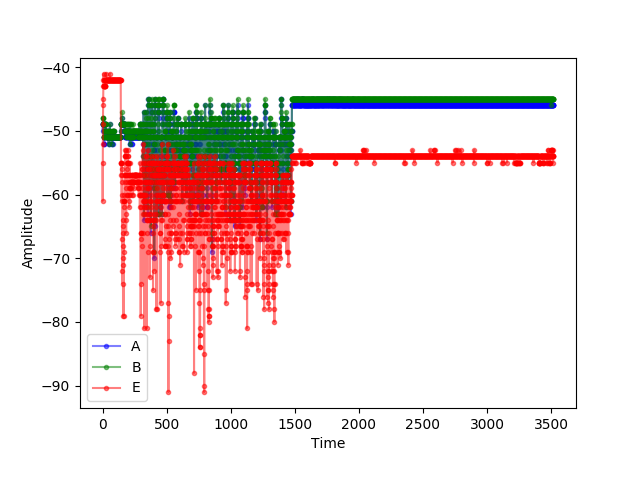
\includegraphics[width=0.65\textwidth ]
		{Bilder/a4-q0-3.png}
		\caption{\textit{Signalstärkenverlauf}}
		\label{fig:4.7}
\end{figure}


\begin{figure}[hbt!]
	\centering
		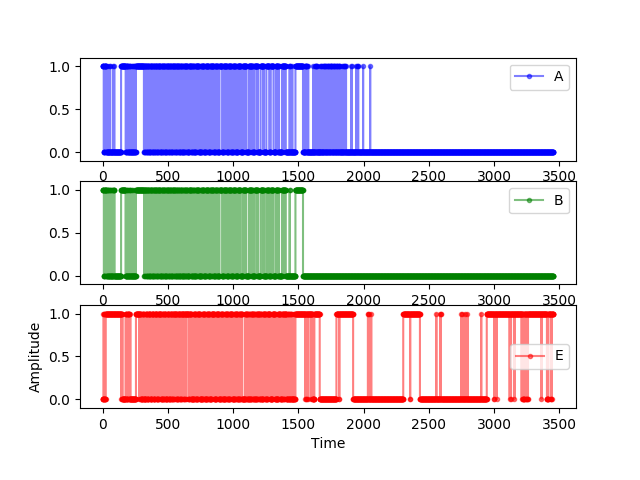
\includegraphics[width=0.65\textwidth ]
		{Bilder/a4-q0-3-1.png}
		\caption{\textit{quant0}}
		\label{fig:4.8}
\end{figure}


\begin{figure}[hbt!]
	\centering
		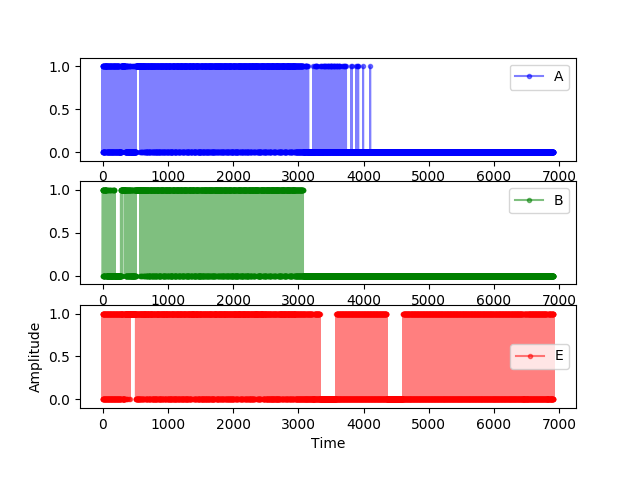
\includegraphics[width=0.65\textwidth ]
		{Bilder/a4-q1-3-1.png}
		\caption{\textit{quant1}}
		\label{fig:4.9}
\end{figure}



\glqq Gibt es einen Zusammenhang zwischen dem Verwendeten
Quantisierer und der Stärke des Angreifers?\grqq
Wie Abbildungen~\ref{fig:4.4} und ~\ref{fig:4.5} zeigen, 
bietet der  \textit{quant0}, also der 
\textit{mean quantizer} dem Angreifer einen leichten Vorteil,
zumindest, wenn die Bedingungen gut sind.
\glqq Welche Rolle spielt die Entfernung des Angreifers 
zu Alice/Bob\grqq
In Abbildungen~\ref{fig:4.8} und ~\ref{fig:4.9} ist klar zu 
erkennen, dass zunehmende Distanz einen Angreifer klar
benachteiligt.
\glqq Welche Rolle spielt die Bewegung im Raum?\grqq
Bewegung im Raum benachteiligt den Angreifer. Die 
Wirkung davon sieht man in Abbildungen~\ref{fig:4.4} 
und~\ref{fig:4.5}.


\subsection*{Repetition Attack}
Wie in der Vorlesung erwähnt wurde, ist es möglich
von einem Angreifer zyklische Bewegungen
auszunutzen, siehe Beispiel Modelleisenbahn.

\begin{figure}[hbt!]
	\centering
		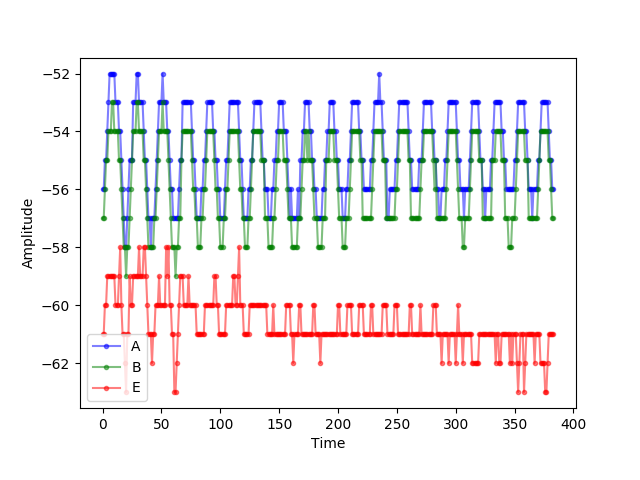
\includegraphics[width=0.65\textwidth ]
		{Bilder/a4-2.png}
		\caption{\textit{Signalstärkenverlauf}}
		\label{fig:4.10}
\end{figure}


\begin{figure}[hbt!]
	\centering
		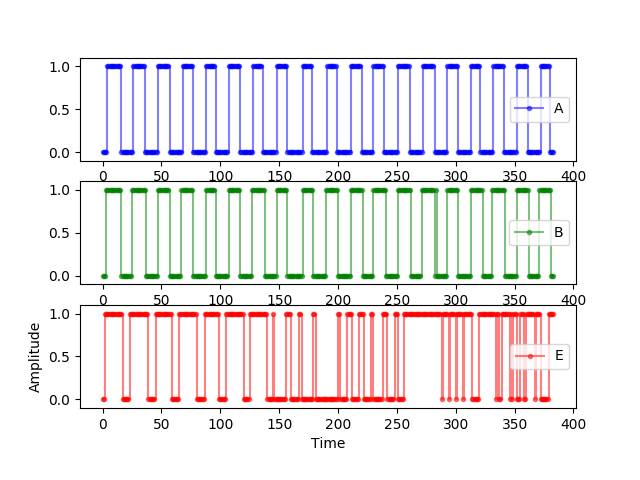
\includegraphics[width=0.65\textwidth ]
		{Bilder/a4-2-q0.png}
		\caption{\textit{quant0}}
		\label{fig:4.11}
\end{figure}


\begin{figure}[hbt!]
	\centering
		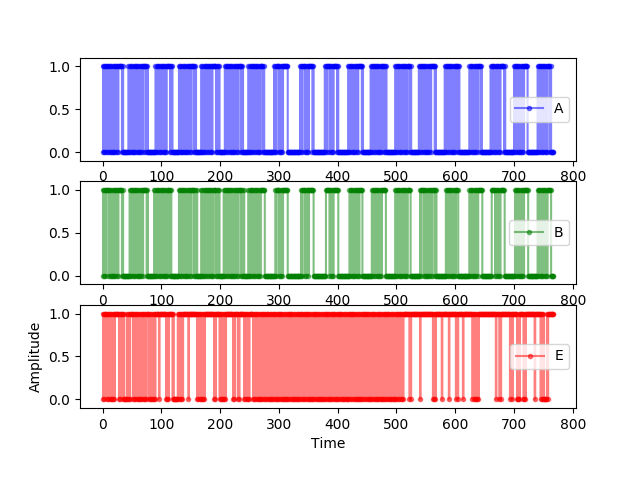
\includegraphics[width=0.65\textwidth ]
		{Bilder/a4-2-q1.png}
		\caption{\textit{quant1}}
		\label{fig:4.12}
\end{figure}


Es sind Muster zu erkennen, wobei 
Eves Muster eigentlich noch gleichmäßiger wäre,
aber die Messbedingungen waren nicht ideal.\\[3mm]
Es gibt erkennbare Unterschiede zwischen den
Quantisierern, wobei Eve \textit{quant0} bevorzugen
würde. Zyklische Bewegungen scheinen tatsächlich 
ausnutzbar zu sein für einen Angreifer. Eve muss dabei
unter anderem die Periode richtig schätzen.


\subsection*{Prediction Attack}

\begin{figure}[hbt!]
	\centering
		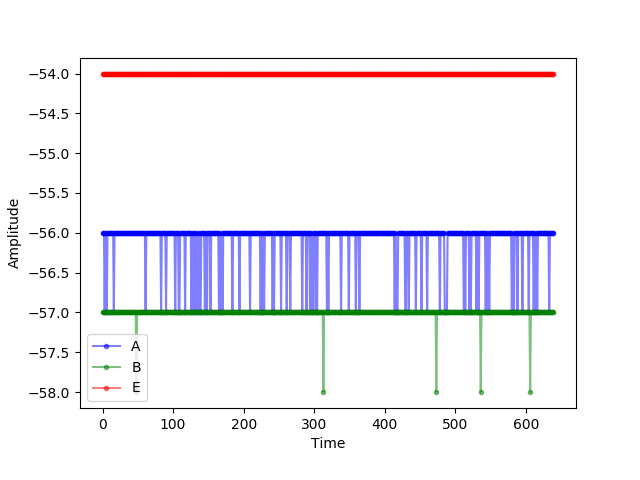
\includegraphics[width=0.65\textwidth ]
		{Bilder/a4-3.png}
		\caption{\textit{Signalstärkenverlauf}}
		\label{fig:4.13}
\end{figure}


\begin{figure}[hbt!]
	\centering
		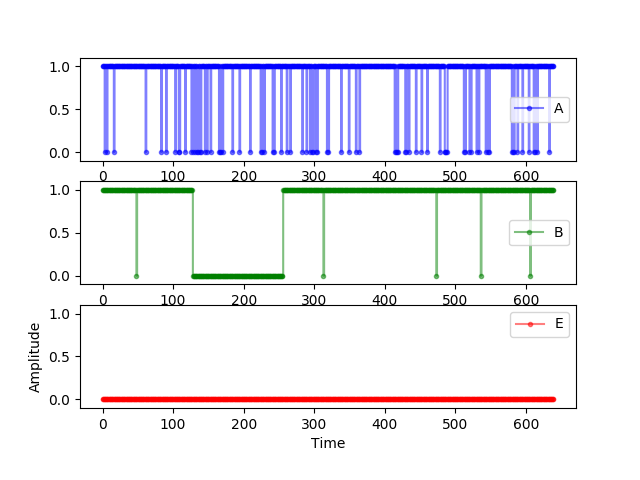
\includegraphics[width=0.65\textwidth ]
		{Bilder/a4-3-q0.png}
		\caption{\textit{quant0}}
		\label{fig:4.14}
\end{figure}


\begin{figure}[hbt!]
	\centering
		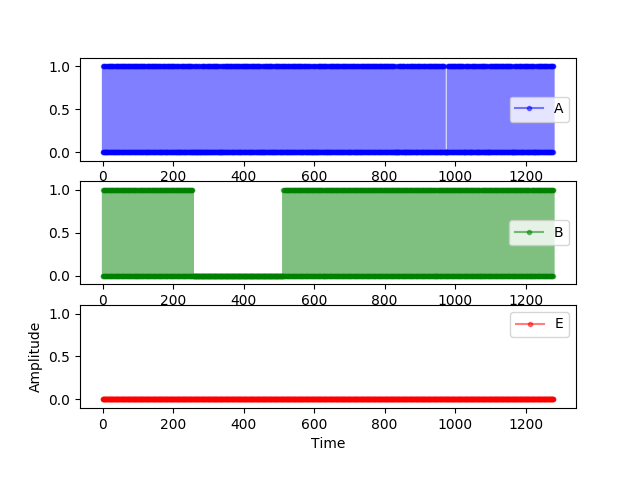
\includegraphics[width=0.65\textwidth ]
		{Bilder/a4-3-q1.png}
		\caption{\textit{quant1}}
		\label{fig:4.15}
\end{figure}

Betrachtet man Abbildungen~\ref{fig:4.14} und 
~\ref{fig:4.15}
kann man zum Entschluss kommen, dass Eve zumindest 
bei \textit{quant0} diese Attacke nutzen könnte um die 
Entropie zwischen Alice und Bob möglichst weit zu 
reduzieren. Alternativ könnte man diesen Angriff als 
\textit{denial-of-service-Attacke} nutzen um eine
erfolgreiche Schlüsseleinigung zwischen Alice und Bob 
zu torpedieren oder sogar zu verhindern. Hier ist
\textit{quant1} deutlich besser, im Sinne von, dass sich
die Quantiserung von Alic und Bob mehr ähneln.
\clearpage

\subsection*{Eigener Angriff}

Idee: Benutze Alufolie und Eisengusspfannen um zu sorgen, dass
Bob möglichst schwach empfängt.


\begin{figure}[hbt!]
	\centering
		\includegraphics[width=0.7\textwidth ]
		{Bilder/a4-4-foto1.jpg}
		\caption{\textit{Vielfach mit Alufolie umwickelt}}
		\label{fig:4.16}
\end{figure}	

\begin{figure}[hbt!]
	\centering
		\includegraphics[width=0.7\textwidth ]
		{Bilder/a4-4-foto2.jpg}
		\caption{\textit{Sakrophag aus Pfannen}}
		\label{fig:4.17}
\end{figure}	

\begin{figure}[hbt!]
	\centering
		\includegraphics[width=0.7\textwidth ]
		{Bilder/a4-4.png}
		\caption{\textit{Signalstärkenverlauf}}
		\label{fig:4.18}
\end{figure}

\begin{figure}[hbt!]
	\centering
		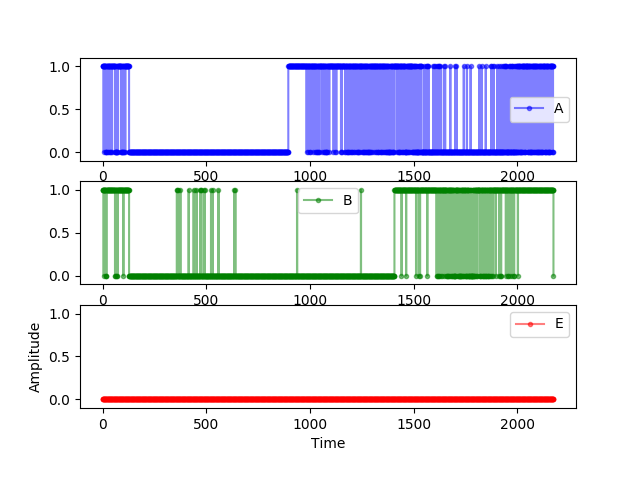
\includegraphics[width=0.7\textwidth ]
		{Bilder/a4-4-q0.png}
		\caption{\textit{quant0}}
		\label{fig:4.18}
\end{figure}
\clearpage


\begin{figure}[hbt!]
	\centering
		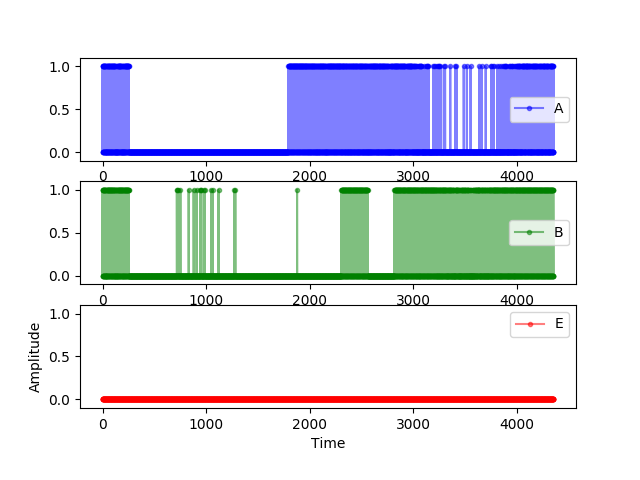
\includegraphics[width=0.7\textwidth ]
		{Bilder/a4-4-q1.png}
		\caption{\textit{quant1}}
		\label{fig:4.19}
\end{figure}

Möglichweise ist es machbar, wenn man diesen Angriff
noch etwas ausfeilt, dass am Ende nur noch Nullen 
quantisiert werden und somit die Schlüsselgenerierung 
manipuliert werden kann. Ansonsten ist es als
\textit{denial-of-service-Attacke} einsetzbar.
Wie zuvor auch, ist hier \textit{quant1} etwas 
besser.